\section{Lossless Compression}
%\subsection{LZ77}
\subsection{LZSS}
\TG{Expand acronym in title}
LZSS~\cite{storer1982data} is a lossless textual compression algorithm. It is a
derivative and improvement of LZ77~\cite{ziv1977universal} which 
compressed data by using previous data as dictionary. There is a sliding window and
a look-ahead buffer applied in both algorithms. Figure~\ref{fig:LZSS} shows the
structure of LZSS. In LZ77 compression algorithm. The algorithm outputs the original
alphabet with empty pointer, e.g. (0, 0)A, if \english{on sub-string} in look-ahead buffer
is found in dictionary~\cite{ziv1977universal}, \english{but it might happen that this
character $A$ and next alphabet compose a string appearing in dictionary}. \TG{Sentence is too long,
and unclear.} LZSS
solves these problems by defining a parameter \emph{MIN\_LENGTH} (size of output
pointers \TG{You should explain what the pointer is}) and only output pointers ($n$, $m$), where $n$ indicates the position
of the first character of the repeating string, $m$ is the length of the
string~\cite{storer1982data}, rather than ($n$, $m$)$C$ in LZ77, where $C$ is
the first first character at sub-string in look-ahead buffer stop finding in
dictionary. The compression \english{process as blow}:

\begin{enumerate}
    \item Find the longest string $str$ which also appears in sliding
    window (dictionary) \TG{Please mind the whitespaces! There is always a space before an opening 
    bracket and after a closing one.} in look-ahead buffer.
    \item Compute pointers $n$ and $m$
    \item Check if the length of $str$ is bigger or equals MIN\_LENGTH. If True,
    it outputs pointers and data stream goes forward length of $str$, else
    outputs the first character in look-ahead buffer and stream goes forward 1
    byte(character).
\end{enumerate}

For instance, assuming that the sliding window and look-ahead buffer are unlimited, and that MIN\_length = 2, 
 string $aaBccDaacEaccFacac$ is
encoded into $aaBccD$(1, 2)$cE$(8, 2)$cF$(8, 2)(8, 2).  \english{also simple to compress
and decompress, and it only decodes by its encoding result (no need to send
dictionary)} \TG{Please make a sentence with a subject and verb.}.

\begin{figure}
    \centering
    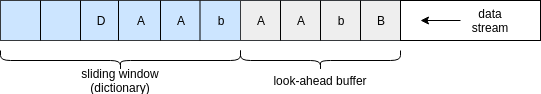
\includegraphics[width=\textwidth]{figures/LZSS.png}
    \caption{Structure of LZSS}
    \label{fig:LZSS}
\end{figure}

\subsection{A-LZSS}
Accelerometer-LZSS~\cite{pope2018accelerometer} is a lossless, dictionary
compression algorithm based on LZSS. As we know, LZSS was introduced
for textual compression, but Pope et al.~\cite{pope2018accelerometer}
implemented LZSS for the devices with limited memory, storage and power. The
authors compressed accelerometer data using A-LZSS which combines LZSS and
entropy coding (Huffman code used in~\cite{pope2018accelerometer}). A flag bit is
assigned to indicate that either an entropy code or a pointer $(n, m)$ is returned \TG{Returned by whom?}. The
pseudo-code of A-LZSS compression algorithm is shown in
Algorithm~\ref{algo:A-LZSS}. \texttt{value\_pointers($S$, $D$)} is a function
that returns the pointer $(n, m)$ which represents the repeating sequence of
elements. Function \texttt{Huffman\_table($x$)} returns the Huffman code of
input $x$. To make stream data in look-ahead buffer and dictionary
move forward \TG{what do you mean by ``move forward?''}, function \texttt{go\_forward($D$, $S$, $x$)} is invoked,
where $x$ indicates the length of movement. The length of look-ahead buffer
$L_{buffer}$ is equal or smaller than the length of dictionary $L_{dict}$,
because the pointer $m$ is not greater than $L_{dict}$. 

In the experiment of Pope et al.~\cite{pope2018accelerometer}, A-LZSS gives
about 1~$\mu$J per byte of energy \TG{do you mean that it saves 1 micro
Joule per bit?} with their CC2650 System-on-Chip. If the data from devices
repeats in high proportion, A-LZSS could be a good choice for energy
saving, because of recording previous data in sliding window as dictionary.
\TG{How does it address the fact that acceleration data is real-valued, hence
there is few exact repetitions of elements?}

\TG{Is the algorithm reproduced from a paper? If yes, please say so. Otherwise,
consider omitting it.}
\begin{algorithm}
\begin{algorithmic}[1]
\Input
    \Desc{$e$}{$\quad \quad \quad $Element in the stream}
    \Desc{$m\_length$}{$\quad \quad \quad $Minimum match length}
    \Desc{$D$}{$\quad \quad \quad $Dictionary in sliding window}
    \Desc{$S$}{$\quad \quad \quad $Sequence of elements in look-ahead buffer}
\EndInput
\Output
    \Desc{tr}{$\quad \quad \quad $Transmitted sequence of bits}
\EndOutput

\State $S$ = $S$ + $e$  \Comment{Add $e$ into look-ahead buffer}
\State $(n, m)$ = value\_pointers($S$, $D$)  \Comment{Compute pointers value}
\If{$m < m\_length$}
    \State $x$ = $S$.first()    \Comment{First element in $S$}
    \State $code$ = Huffman\_table($x$)
    \State go\_forward($D$, $S$, 1) \Comment{Move stream forward 1 element}
    
    \State tr.flag(True)    \Comment{Assign flag bit}
    \State tr.bits($code$)  \Comment{Append $code$ in tr in bits}
    
\ElsIf{$m$ == $S$.length}   \Comment{$S \subseteq D$}
    \State \Return null     \Comment{No transmitted data}
    
\Else                       \Comment{$S \not\subseteq D$, $S-e \subset D$}
    \State go\_forward($D$, $S$, $m$) \Comment{Move stream forward m element}
    
    \State tr.flag(False)
    \State tr.bits( $(n-1, m-1)$ )  \Comment{Write data in bits}
\EndIf

\If{tr.length $\geqslant m$} \Comment{Compressed result needs more bits/bytes}
    \State tr.clear()
    \State $seq$ = $S$.subset($m$) \Comment{subset of $m$ first elements}
    \State tr.flag(False)
    \State tr.bits($seq$)   \Comment{Transmit original data}
\EndIf
\State \Return tr

\end{algorithmic}
\caption{pseudo-code of A-LZSS Algorithm}
\label{algo:A-LZSS}
\end{algorithm}

\subsection{LZW}
LZW~\cite{welch1984technique} is a dictionary-based lossless compression
algorithm, derived from LZ78~\cite{ziv1978compression}. Different with LZSS
which saves dictionary in a sliding window, LZW uses a length-variable
dictionary (map table) to record the previous data elements. An initial
dictionary which contains all characters (e.g. ASCII Table) is needed for
compression~\cite{welch1984technique}, and two variables $P$ and $C$ are
maintained in LZW. $P$ (Previous sequence) \english{indicates the sequence already in hand}
but is not compressed, $C$ (Current character) is the new element received. The
Algorithm of LZW is shown here:

\begin{enumerate}
    \item Initialize dictionary. Assign $P$ and $C$ to empty.
    \item Read new element $e$, assign $C$ = $e$.
    \item Find $P+C$ in dictionary. If found it, assign $P$ = $P+C$. Otherwise
    output the index of $P$ in dictionary, add entry of $P+C$ in dictionary and
    update $P$ = $C$.
    \item Go to step 2 if input data is not empty.
\end{enumerate}

A dictionary entry shall be created and appended into dictionary for each
sequence of data has never seen. According to this feature, the result after
compression by LZW is self-explaining~\cite{welch1984technique}. It means
that the initial dictionary and the encoding result are the only things
needed for decoding process~\cite{welch1984technique}. But LZW can not fit
resource-constrained IoT devices exactly, because of its extended dictionary.
\TG{Also, can it encode real-valued streams?}

\subsection{S-LZW}

S-LZW was introduced by Sadler et al.~\cite{sadler2006data}. It adapts LZW to
sensor nodes. There are several challenges for using LZW in sensor devices:
\begin{enumerate}
    \item \english{What is solution for packet loss in sensor network.}
    \item How to address dictionary extension.
    \item What strategy is applied when dictionary is full, if we fix the size
    of dictionary.
\end{enumerate}

As we know, the decompression of LZW depends on the previous entries in the
table, thus, the decoding process makes mistakes when network packets have been lost
over transmission. To address this issue, S-LZW separates the data stream into small
blocks (512~B), so that each block is independent and not affected by
others~\cite{sadler2006data}. Because of limited storage and memory of sensor
nodes, the dictionary stored has fixed size, but it may cause decrements of
compression ratio. In fact, that is not a problem if the data blocks for
compression are small enough, as the dictionary won't be filled until we compress
whole data in block. In~\cite{sadler2006data}, two strategies are presented to address
full dictionaries: (1) freeze the dictionary and use it for rest stream data in block,
or (2) reset it and start from scratch~\cite{sadler2006data}. S-LZW applies the first
strategy, because the former provides faster processing speed and better
compression ratio than the later. S-LZW adds a hash-indexed table,
Mini-Cache (MC), to store recently used and created dictionary entries for the
specific scenario that sensor data might repeats itself in short intervals. A
example of MC is shown in Table~\ref{table:MC}. The output of S-LZW adds one
extra flag bit to distinguish the output is encoded by either dictionary or
Mini-Cache, e.g. '0' bit indicates encoded from dictionary, '1' means encoded
from MC. Algorithm~\ref{algo:S-LZW} shows the pseudo-code of S-LZW-MC.
\TG{Same question on the algorithm: is it reproduced from a paper? If yes, say so.}
\begin{table}[]
    \begin{minipage}{.45\textwidth}
        \centering
        \begin{tabular}{|l|l|}
        \hline
        \multicolumn{2}{c}{Dictionary}  \\ \hline
        Index           & Entry         \\ \hline
        256             & AA            \\ 
        257             & AB            \\ 
        258             & BC            \\ 
        259             & BA            \\
        260             & AAA           \\
        261             & AAAB          \\
        262             & CA            \\
        \hline
        \end{tabular}
    \caption{Dictionary}
    \end{minipage}
    \hfill
    \begin{minipage}{.45\textwidth}
        \centering
        \begin{tabular}{|l|l|}
        \hline
        \multicolumn{2}{c}{Mini-Cache}  \\ \hline
        Index        & Dict\_index      \\ \hline
        0            & 261              \\
        1            & 258              \\
        2            & 262              \\
        3            & 256              \\
        \hline
        \end{tabular}
    \caption{Dictionary}
    \end{minipage}
   
    \caption{Example of using MC}
    \label{tab:MC}
\end{table}

\begin{algorithm}
\begin{algorithmic}[1]
\Input
    \Desc{$P$}{$\quad $Previous sequence}
    \Desc{$C$}{$\quad $Current element received}
    \Desc{$D$}{$\quad $Dictionary}
    \Desc{$MC$}{$\quad $Mini-Cache table}
\EndInput
\Output
    \Desc{tr}{$\quad $Transmitted sequence of bits}
\EndOutput

\State $P_c$ = $P$ + $C$
\If{$P_c \not\in D$}
    \If{$P \in MC$}
        \State tr.flag(True)    \Comment{Assign flag bit}
        \State $code$ = $MC$.encode($P$)    \Comment{Encode data using MC}
        
    \Else   \Comment{$P \in D$}
        \State tr.flag(False)
        \State $code$ = $D$.encode($P$)
        \State $MC$.add($P$)    \Comment{Add new entry into MC}
    \EndIf
    \State $D$.add($P_c$)
    \State $P$ = $C$
    
    \State tr.bits($code$)
    \State \Return tr
\Else       \Comment{$P_c$ is not in neither $D$ nor $MC$}
    \State $P$ = $P+C$
    \State \Return null \Comment{No transmitted data}
\EndIf

\end{algorithmic}
\caption{Algorithm of S-LZW with Mini-Cache}
\label{algo:S-LZW}
\end{algorithm}

By using Mini-Cache in S-LZW, the compression ratio improves, because of
representing data sequences by $O(\log N + 1)$ instead of $O(\log D)$,
where $N$ is the size of Mini-cache, $D$ is the size of the dictionary.
In~\cite{sadler2006data}, S-LZW offers energy savings, and it reduced
energy consumption on average by over 2.5$\times$.


\subsection{LEC}
LEC algorithm was first proposed by Marcelloni et
al.~\cite{marcelloni2008simple}, which is a approximated version of
exponential-Golomb code~\cite{teuhola1978compression}. In
paper~\cite{marcelloni2008simple}, authors measured temperature and humidity by
sensors and compressed data by using LEC. It uses very small dictionary whose
size is determined by the number of the bits after ADC
converter~\cite{marcelloni2008simple,marcelloni2009efficient}.  For instance, in
a sensor node, a measure $m_i$ is gained and converted into numeral value $r_i$
represented on $R$ bit by ADC. For each new data point $r_i$, LEC compute the
difference of adjacent points $d_i$ = $r_i$ - $r_{i-1}$, in order to compute
$d_0$, the $r_{-1}$ equals the central value among $2^R$. The residue $d_i$
encoded by entropy encoder, and represented as a bit sequence in 2 parts $s_i |
a_i$ , where $s_i$ is the value of the bits needed to represent the difference
$d_i$, and $a_i$ represent $d_i$ based on special rule:
\begin{enumerate}
    \item If $d_i = 0$, $a_i$ is not present.    
    \item If $d_i > 0$, $a_i$ is the binary expression of $n_i$ low-order bits
    of the $d_i$
    \item If $d_i < 0$, $a_i$ is the binary expression of $n_i$ low-order bits
    of the two's complement representation of ($d_i$ - 1)
\end{enumerate}

In the paper~\cite{marcelloni2008simple}, the authors generated the $s_i$ from
$n_i$ by Huffman coding. Let's say the $s_i$ is the representation at $n_i$ in
the Huffman code, $n_i$ = $(\log{_2}{\left|{b_i}\right|} +
1)$~\cite{li2016temporal} and $n_i \leq R$. Table~\ref{table:LEC} is used in
paper~\cite{marcelloni2009efficient}. From the Table~\ref{table:LEC}, it
supports R+1 groups($n_i$) and each group $s_i$ contains $2^{n_i}$ numeral
value.  
\begin{table}[]
\begin{tabular}{|l|l|l|}
\hline
$n_i$ & $s_i$        & $d_i$                                  \\ \hline
0     & 00           & 0                                      \\ 
1     & 010          & -1, +1                                 \\
2     & 011          & -3, -2, +2, +3                         \\
3     & 100          & -7, ..., -4, +4, ..., +7               \\
4     & 101          & -15, ..., -8, +8, ..., +15             \\
5     & 110          & -31, ..., -16, +16, ..., +31           \\
6     & 1110         & -63, ..., -32, +32, ..., +63           \\
7     & 11110        & -127, ..., -64, +64, ..., +127         \\
8     & 111110       & -255, ..., -128, +128, ..., +255       \\
9     & 1111110      & -511, ..., -256, +256, ..., +511       \\
10    & 11111110     & -1023, ..., -512, +512, ..., +1023     \\
11    & 111111110    & -2047, ..., -1024, +1024, ..., +2047   \\
12    & 1111111110   & -4095, ..., -2048, +2048, ..., +4095   \\
13    & 11111111110  & -8191, ..., -4096, +4096, ..., +8191   \\
14    & 111111111110 & -16383, ..., -8192, +8192, ..., +16383 \\
\hline
\end{tabular}
\caption{The dictionary table used in the experiments~\cite{marcelloni2009efficient}}
\label{table:LEC}
\end{table}
 
\subsection{S-LEC}
S-LEC Algorithm is a extension and improvement of LEC Algorithm by Li et
al.~\cite{li2016temporal}. Same with LEC, it encodes residues in compression
process, because of the correlation characteristic of sensor stream, e.g. the
different of stream data unlikely be too large. In LEC, the result after
encoding has two parts $s_i$ and $ a_i$, and the $s_i$ part shell cause
information redundancy, if a set of residues are in same group which means
repeated group index $s_i$. S-LEC reduces the size of representation by
exploiting the correlation amount adjacent residues. The main idea is using a
extra two bits of sequential code $b_i$ to present the positional relationship
of groups of adjacent residues~\cite{li2016temporal}. The encoding result
$s_i|a_i$ is replaced by $b_i|s_i|a_i$, but the group index $s_i$ shell be
omitted if two adjacent residues are in same group or neighboring group. Assume
the number of the group in table is K, the $b_i$ is defined
as~\cite{li2016temporal}: 

\begin{enumerate}
    \item $b_i$ = 00, if $s_i$ = $s_{i-1}$
    \item $b_i$ = 01, if $n_i$ = $n_{i-1}$ - 1($n_{i-1} \geqslant 1$), or $n_i$
    = $n_{i-1}$ + 2($n_{i-1}$ = 0)
    \item $b_i$ = 10, if $n_i$ = $n_{i-1}$ - 1($n_{i-1} \leqslant K$), or $n_i$
    = $n_{i-1}$ - 2($n_{i-1}$ = K)
    \item $b_i$ = 11, otherwise. The representation $b_i|s_i|a_i$ is required. 
  \end{enumerate}

When the $b_i$ equals 11, the representation need more bits than LEC result,
because of extra $b_i$. S-LEC proposed some context situations to solve this
problem. In paper~\cite{li2016temporal}, the groups is divided into three
clusters: $C_1$ = {$n_i$|$i$ = 0, 1, 2, 3}, $C_2$ = {$n_i$|$i$ = 4, 5} and 
$C_3$ = {$n_i$|$i$ = 6, ..., K}. The idea of reducing group code as
follow~\cite{li2016temporal}:

\begin{enumerate}
    \item $s_i$ remove the first "1", If $n_{i-1} \in C_1$
    \item $s_i$ remove the first two "1"s, If $n_{i-1} \in C_2$
    \item $s_i$ remove the first three "1"s, If $n_{i-1} \in C_3$
\end{enumerate}
S-LEC gives better Compression ratio then LEC when they are in same SME(Square
Mean Error)~\cite{li2016temporal}. We need to save the table into memory when we
uses these two algorithms, and in order to improve compression ratio as much as
possible, it is necessary to encode $n_i$ by prefix code method base on the
elements distribution.
